%
% methods_data_transmission.tex
%

\subsection{Server-Client Handshake}
Any web-based data visualization involves some communication between the server and the client in the form of requests for data and responses including transmitted data.  In order to effectively communicate and exchange visualizable data, the server and the client must “speak a common language” by offering requests and responses in a predictable format.  Our architecture allows the client and the server to accommodate changes to the available dataset list while still maintaining a standard communication format.  This is accomplished using a simple server-client handshake as is visualized in Figure \ref{fig:server-client-handshake}.  The handshake opens with the client page loading and emitting a connection event.  The server catches this event and generates a list of available datasets typically populated using a configuration file and/or database query.  This list is then transmitted back to the client.  The client receives the list and since it knows what datasets are available for querying, it will form a response.  The server filters this request using it’s configuration data to prevent unpermitted data accesses.  The server will then query using the filtered dataset list and form a response to the client.  The response will be formatted such that each requested dataset is a JSON object key used to access a list of data items for that data set.  Finally, the client receives the data and can dynamically interpret it using the dataset list that it has received at the beginning of the handshake. This simple handshake system allows the client and server to dynamically include new datasets or remove old datasets without codebase changes. \par
\begin{figure}
    \centering
    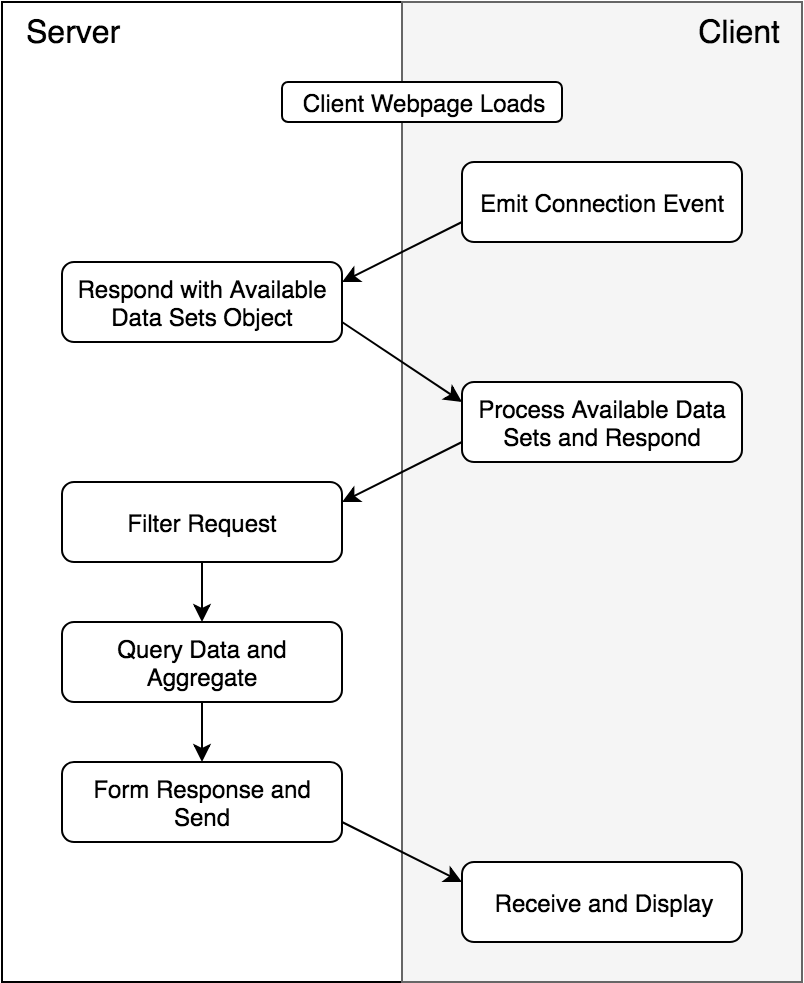
\includegraphics[width=4in]{images/ServerClientHandshake.png}
    \caption{Server-Client Handshake}
    \label{fig:server-client-handshake}
 \end{figure}
Beestream includes a concrete implementation of this data transmission system.  The implementation utilizes Socket.io to handle bidirectional communications.  All data is transmitted in JSON format.  The implementation follows the architecture almost directly, differing only in the original dataset list handshake step.  During this step, the server not only responds with a list of available data sets, but also a list of available datetimes and other fields necessary to populate a data selection widget.  The client will then transmit a set of selected datasets as well as a range of data points to the client in the next response.  The format for this communication is standardized throughout the application.  Using this method, we can allow the user to filter the dataset and form their data request. \par
